% This file was created by matlab2tikz.
%
\documentclass[tikz]{standalone}
\usepackage[T1]{fontenc}
\usepackage[utf8]{inputenc}
\usepackage{pgfplots}
\usepackage{grffile}
\pgfplotsset{compat=newest}
\usetikzlibrary{plotmarks}
\usetikzlibrary{arrows.meta}
\usepgfplotslibrary{patchplots}
\usepackage{amsmath}

\newlength\figureHeight \setlength{\figureHeight}{6cm}
\newlength\figureWidth \setlength{\figureWidth}{10cm}
\begin{document}
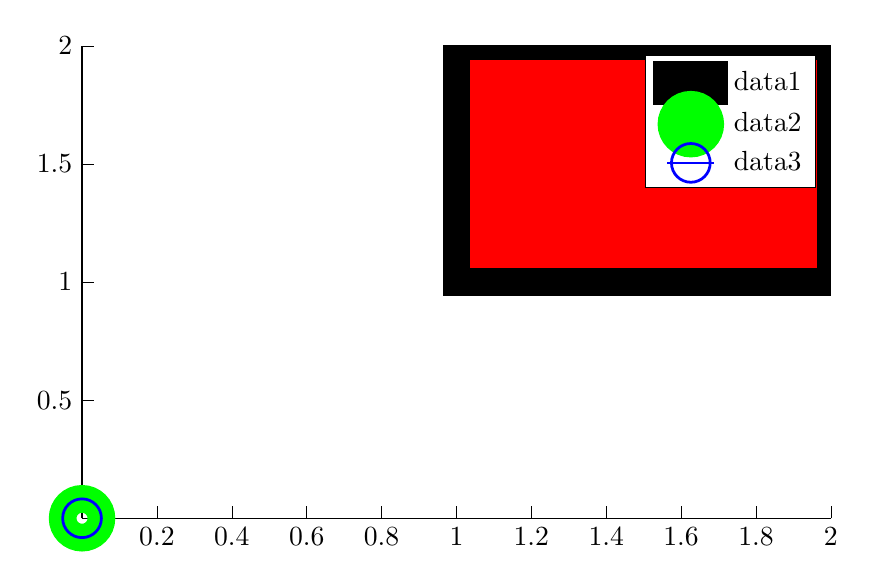
\begin{tikzpicture}

\begin{axis}[%
width=0.951\figureWidth,
height=\figureHeight,
at={(0\figureWidth,0\figureHeight)},
scale only axis,
every outer x axis line/.append style={black},
every x tick label/.append style={font=\color{black}},
every x tick/.append style={black},
xmin=   0,
xmax=   2,
every outer y axis line/.append style={black},
every y tick label/.append style={font=\color{black}},
every y tick/.append style={black},
ymin=   0,
ymax=   2,
axis background/.style={fill=white},
axis x line*=bottom,
axis y line*=left,
legend style={legend cell align=left, align=left, draw=black}
]

\addplot[area legend, line width=10.0pt, draw=black, fill=red]
table[row sep=crcr] {%
x	y\\
   1	   1\\
   1	   2\\
   2	   2\\
   2	   1\\
}--cycle;
\addlegendentry{data1}

\addplot [color=green, line width=10.0pt, draw=none, mark size=7.0pt, mark=o, mark options={solid, green}]
  table[row sep=crcr]{%
   0	   0\\
};
\addlegendentry{data2}

\addplot [color=blue, line width=1.0pt, draw=none, mark size=7.0pt, mark=o, mark options={solid, blue}]
  table[row sep=crcr]{%
   0	   0\\
};
\addlegendentry{data3}

\end{axis}
\end{tikzpicture}%
\end{document}